\documentclass{exam}

\usepackage{units} 
\usepackage{graphicx}
\usepackage[fleqn]{amsmath}
\usepackage{cancel}
\usepackage{float}
\usepackage{mdwlist}
\usepackage{booktabs}
\usepackage{cancel}
\usepackage{polynom}
\usepackage{caption}
\usepackage{fullpage}
\usepackage{xfrac}
\usepackage{enumerate}

\newcommand{\degree}{\ensuremath{^\circ}} 
\everymath{\displaystyle}

\printanswers

% \begin{figure}[H]
%   \centering
%   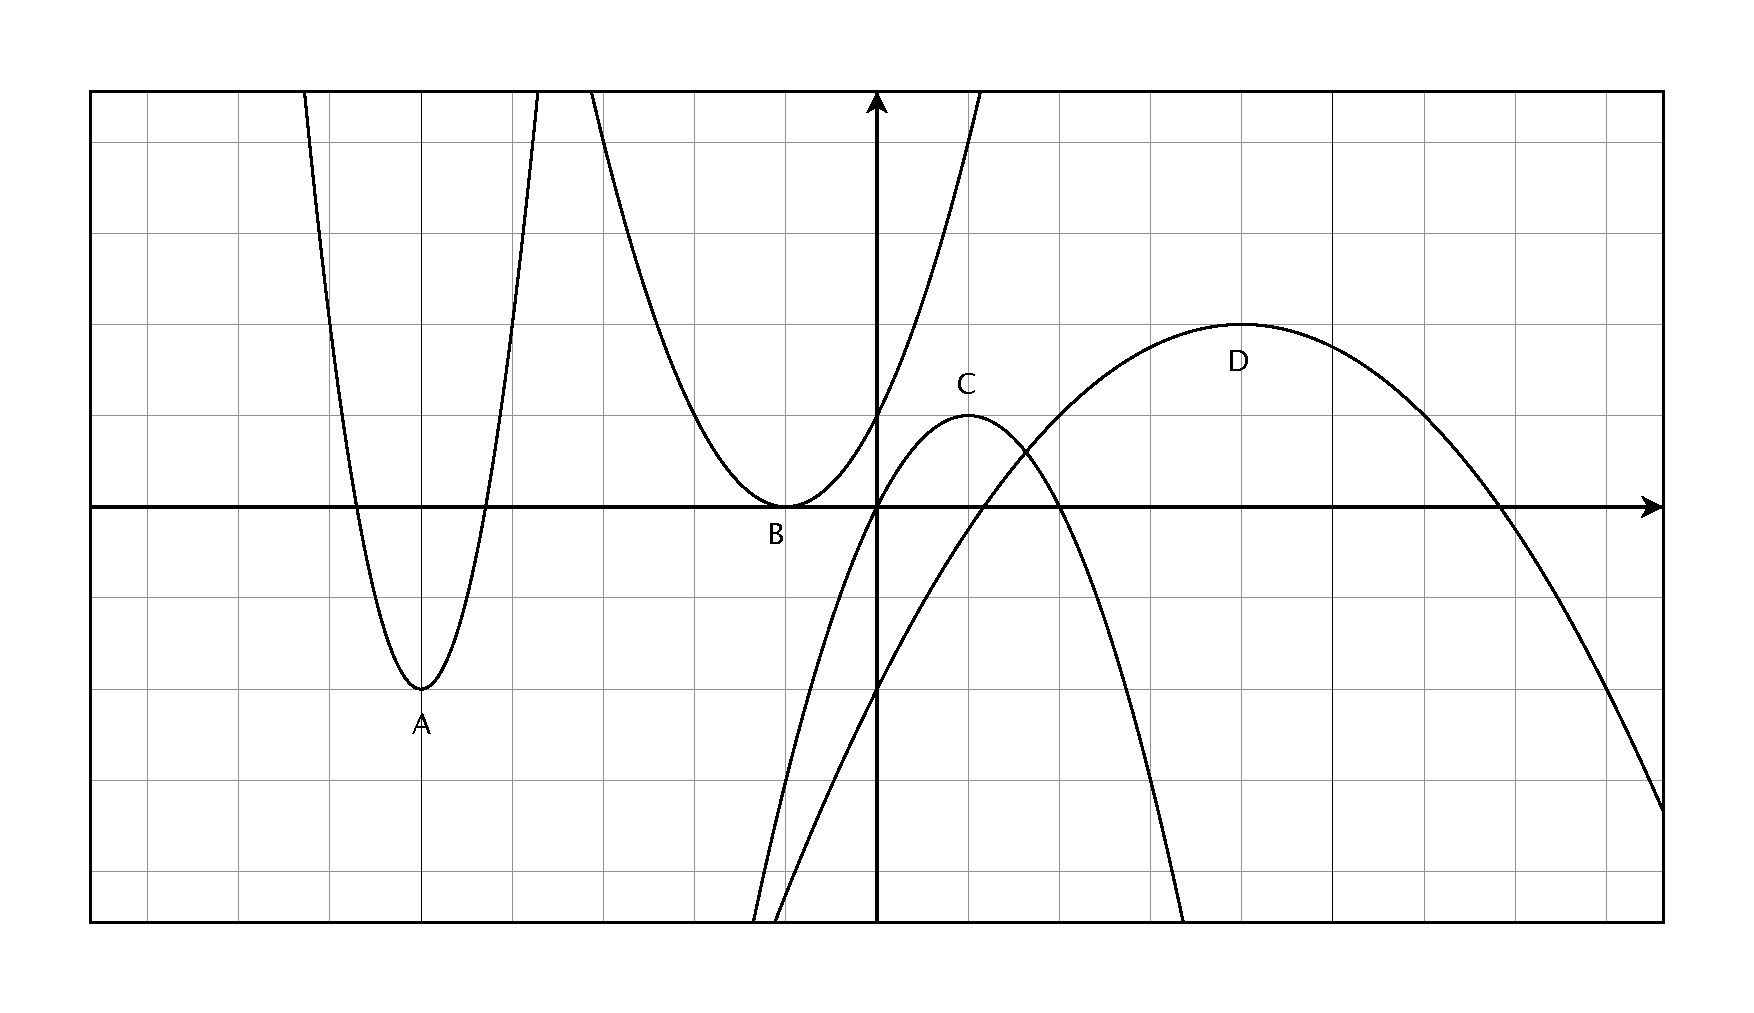
\includegraphics[scale=.3]{problem_7.eps}
%   \caption*{Problem 7}
% \end{figure}

% \begin{tabular}{cc}
% \toprule
% period & amplitude \\
% \midrule
%   $\pi$ & $2$ \\
% \bottomrule
% \end{tabular}

\title{Math 141 Notes \\ Section 3.5}
\date{May 1, 2013}

\begin{document}

\maketitle
\tableofcontents

\section{Fundamental Theorem of Algebra}

Every polynomial with complex coefficients has at least one complex zero.  Since real numbers are also complex numbers,
this also applies to polynomials with real coefficients.

\section{Complete Factorization Theorem}
Every polynomial can be factored into linear factors multiplied by a constant:
\[
  P(x) = a(x - c_1)(x - c_2) \cdots (x - c_n)
\]

Proof:
\begin{itemize*}
  \item From FTA, there is at least one zero, so $P(x) = (x - c_1) Q(x)$, where $Q(x)$ is one lower degree.
  \item Keep going until the final Q(x) is a constant instead of a linear factor
\end{itemize*}

\section{Zeros Theorem}
Every polynomial of degree $n \geq 1$ has exactly $n$ zeros, counting multiplicity.

Proof:
\[
  P(x) = a(x - c_1)(x - c_2) \cdots (x - c_n) \\
\]

All of the $c_i$s are zeros and there are $n$ $c_is$, so $P$ has at least $n$ zeros.

If $c$ is a zero, $P(c) = 0$:
\[
  a (c - c_1)(c - c_2) \cdots (c - c_n) = 0
\]
    
$c$ must equal one of the $c_i$s since $a \neq 0$, so $P$ also has at most $n$ zeros.

\section{Conjugate Zeros Theorem}

\subsection{Description}

If a polynomial, $P$ has only real coefficients, and if the complex number $z$ is a zero, of $P$, then
$\bar{z}$ is also a zero of $P$.

\subsection{Proof}

Suppose $z$ is a zero, so $P(z) = 0$.  Find $P(\bar{z})$:

\begin{align*}
  P(\overline{z}) &= a_n (\overline{z})^n \cdots a_0 \\
                  &= a_n \overline{z^n} \cdots a_0                       \tag{1} \\
                  &= \overline{a_n} \overline{z^n} \cdots \overline{a_0} \tag{2} \\
                  &= \overline{a_n z^n} \cdots \overline{a_0}            \tag{1} \\
                  &= \overline{a_n z^n \cdots a_0}                       \tag{3} \\
                  &= \overline{P(z)} \\
                  &= 0 \\
\end{align*}

notes:
\begin{enumerate}
  \item $\overline{x} \cdot \overline{y} = \overline{xy}$
  \item the conjugate of a real number is also real
  \item $\overline{x} + \overline{y} = \overline{x + y}$
\end{enumerate}

\subsection{Examples}

\begin{enumerate}
  \item Find an polynomial of degree 3 with roots $2$ and $1 + i$.
    \[
      f(x) = x^3-4 x^2+6 x-4
    \]

  \item Find an polynomial of degree 4 with roots $\pm 2$ and $\pm 2i$.
    \[
      f(x) = x^4 - 16
    \]
\end{enumerate}

\pagebreak

\section{Linear and Quadratic Factors Theorem}

\subsection{Description}
An {em irreducible quadratic} is a quadratic that can't be factored into real numbers.

Every polynomial with real coefficients can be factored into a product of linear and irreducible quadratic factors with
real coefficients.

\subsection{Proof}

Multiplying conjugate pair factors gives a quadratic with real coefficients:
\begin{align*}
  c                         &= a + bi \\
  (x - c)(x - \overline{c}) &= x^2 - 2ax + (a^2 + b^2) \\
\end{align*}

If $P(x) = a(x - c_1)(x - c_2) \cdots$, the conjugate pairs turn into irreducible quadratics and the other factors are
linear.

\subsection{Examples}

\[
  x^3-2 x-4 = (x-2) \left(x^2+2 x+2\right)
\]

\end{document}
